\section{Intelligenza Artificiale}
Il termine intelligenza artificiale ha avuto un processo di evoluzione considerevole negli ultimi anni.
Molte definizioni descrivono l'intelligenza artificiale come la capacità di elaboratori o sistemi robotici di poter eseguire operazioni come l'apprendimento o il prendere decisioni in modo analogo alla capacità degli umani \cite{MWDict,CollinsDict}
Quello che rende l'intelligenza artificiale estremamente diffusa nel mondo accademico e industriale è la sua capacità evolutiva, in particolare nell'ultimo decennio, trasformando questa definizione a tal punto da renderla incompleta.
Una definizione che evidenzia maggiormente lo scopo di questa disciplina è stata fornita da John McCarthy \cite{mccarthy2004}, la quale viene definita come:
\begin{quote}
\textit{    La scienza e l'ingegneria di rendere le macchine intelligenti e in particolare i programmi intelligenti. E' correlata a task simili all'utilizzo del computer per la comprensione dell'intelligenza umana, ma l'intelligenza artificiale non deve limitarsi ai metodi che sono osservabili biologicamente.}
    \end{quote}
Sebbene lo scopo di questa disciplina era inizialmente quello di poter permettere alle macchine di imitare la capacità intellettuale degli umani, ora si ritiene che essa possa andare oltre.
L'attuale definizione porta alla definizione di questa disciplina su più livelli \cite{wiki:Artificial_intelligence}:
\begin{itemize}
    \item \textbf{Artificial Narrow Intelligence:} applicazione dell'intelligenza artificiale al fine di avere la capacità di applicare intelligenza in un determinato problema.
    \item \textbf{Artificial General Intelligence:} applicazione dell'intelligenza artificiale al fine di avere la capacità di applicare intelligenza su tutti i problemi su cui un essere umano può applicare.
    \item \textbf{Artificial Super Intelligence: } applicazione dell'intelligenza artificiale al fine di superare le capacità di applicare intelligenza su tutti i problemi rispetto a un essere umano.
\end{itemize}

\subsection{Machine Learning}

Il machine learning è uno dei rami dell'intelligenza artificiale utilizzato dalle industrie. Esso rappresenta l'insieme di tecniche, metodologie e teorie utili a consentire agli elaboratori di poter apprendere utilizzando metodi matematico-computazionali \cite{Michalski1984MachineL}.
Quest'area di ricerca ha l'intento di permettere alle macchine di riconoscere pattern e creare un sistema di decisioni basandosi sui dati.
In particolare può essere definita come l'applicazione di migliorare sull'esecuzione di un task $T$ rispetto alla misura di performance $P$ basandosi sull'esperienza $E$.
Un tipico esempio per la rappresentazione di un sistema di machine learning è quello del filtraggio delle e-mail spam, come raffigurato in Tabella \ref{tab:spam_example}.


\begin{table}[]
    \centering
    \begin{tabular}{|c|p{7cm}|}
        \hline
         Task (T) & Identificare le e-mail che gli utenti non desiderano ricevere.  \\
         \hline
         Performance (P) & Percentuale di e-mail spam che sono filtrate e percentuale di e-mail che sono incorrettamente filtrate.\\
         \hline
         Esperienza (E) & Database di e-mail etichettate come e-mail spam e o non-spam.\\
        \hline
    \end{tabular}
    \caption{Esempio di rappresentazione di un sistema di Machine Learning}
    \label{tab:spam_example}
\end{table}
A seconda della rappresentazione del task $T$ e dell'esperienza $E$ che si ha a disposizione, è possibile utilizzare diverse tecniche di machine learning, classificabili nelle seguenti tipologie \cite{lecun2015deep}:
\begin{itemize}
    \item Apprendimento supervisionato (Supervised Learning): Questa tipologia di tecnica ha l'obiettivo di creare un modello di predizione utilizzando come input i dati costituiti sia da un insieme di attributi, sia da un attributo target. Attraverso la definizione di questi dati, il modello cerca di comprendere il valore dell'attributo obiettivo (target) su nuove osservazioni, non elaborate prima. Per questo tipo di apprendimento esistono due tipologie che si differenziano in base al tipo di predizione che si vuole effetturare sull'attributo target: classificazione e regressione.
    La prima tipologia si basa sul predire la classe di appartenenza tra le diverse istanze di oggetti, la seconda, anche se concettualmente simile alla classificazione, si basa sul predire il valore dell'attributo target su insieme di valori continui.
    \item Apprendimento non supervisionato (Unsupervised Learning): A differenza delle tecniche di apprendimento supervisionato, questa tipologia prevede l'utilizzo di dati non classificati e che appartengono quindi a strutture sconosciute. In particolare, il termine \textit{non supervisionato} deriva dalla caratteristica che i dati non sono etichettati secondo un determinato attributo target. Una tipica applicazione per le tecniche di questa tipologia sono i task di clustering: lo scopo è quello di effettuare un'analisi al fine di identificare nell'insieme di dati dei sottinsieme (detti \textit{cluster}), la quale suddivisione fornisce informazione sul sott'insieme dei dati.
    \item Apprendimento per rinforzo (Reinforcement Learning): Le tecniche di apprendimento per rinforzo prevedono l'estrazione dei dati tramite l'interazione del modello con l'ambiente. Il modello esegue un'azione e riceve un feedback dall'ambiente il quale sarà fonte di informazioni utile alla decisione di quale sarà la prossima azione da eseguire. In questo modo, il modello comprende quali sono le migliori azioni al fine di massimizzare il risultato. In particolare, attraverso la definizione di politiche di premialità e di penalità, il modello indirizza la serie di scelte al fine di ottenere il più alto punteggio.
\end{itemize}


Per la definizione di un modello di machine learning è necessario andare a pianificare il processo di apprendimento, come illustrato in Figura \ref{fig:ml_process}.
Il processo tipicamente utilizzato prevede quindi di partire dall'estrazione dei dati. La scelta dei dati da estrarre dipende dal problema che si affronta e dalla tipologia di tecnica che si utilizza. 
La qualità dell'insieme dei dati viene poi analizzata. In questa fase saranno identificati tutte le problematiche dei dati che possono comportare al degrado della qualità del modello, come la presenza di \textit{missing value} o \textit{outlier} della distribuzione.
Successivamente i dati vengono trasformati e, in particolare, dalla forma grezza iniziale dei dati sarà avviato un processo di \textit{feature engineering}, il quale ci consente di poter estrarre la serie di attributi che aumentano il livello di rappresentazione e dettaglio dei dati.
Alla fine di questa fase, i dati assumeranno una forma strutturata in base al task da elaborare. Nel caso di utilizzo di una tecnica di apprendimento supervisionato, dai dati sarà estratto un insieme di osservazioni dove ognuna è rappresentata dalla descrizione di un insieme di attributi (definite in letteratura come \textit{features}) e da un'attributo target su cui andare a basare il nostro task di classificazione.
Una volta che i dati sono stati strutturati, è possibile andare a selezionare la tecnica di machine learning di cui si ha bisogno, i parametri di configurazione del modello finale, e infine effettuare l'addestramento attraverso l'analisi di una parte dell'insieme dei dati definita come \textit{training set}.
Il risultato della fase precedente quindi sarà un modello capace di poter effettuare elaborazione del task. Quindi, questo modello sarà soggetto a un processo di validazione al fine di poter misurare le sue performance e verificare la qualità del modello.

\begin{figure}[h]
    \centering
    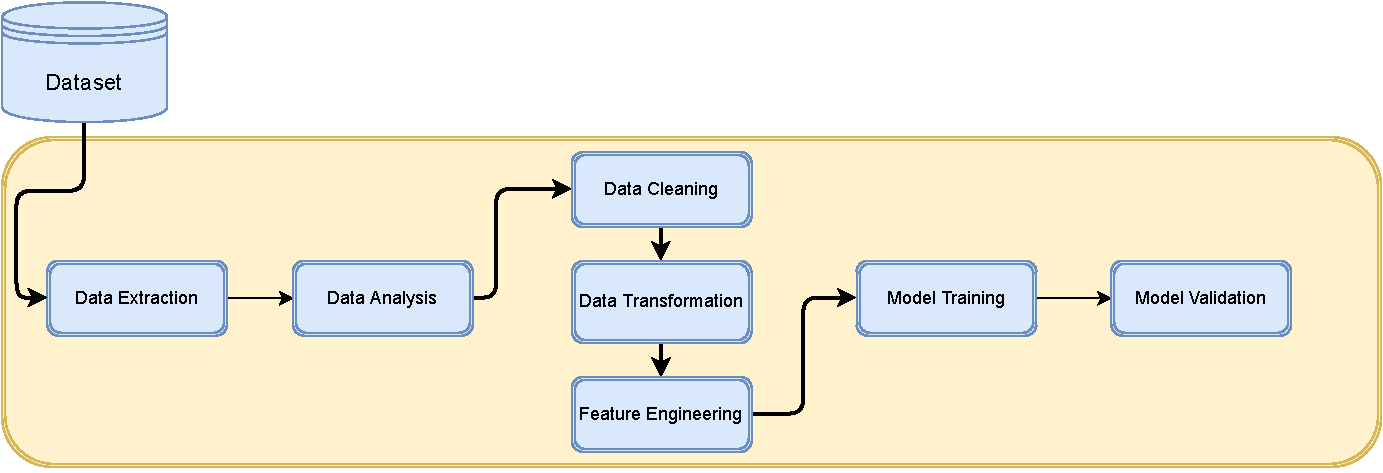
\includegraphics[width=\textwidth]{Figure/Background/ML_Pipeline-2.pdf}
    \caption{Typical Machine Learning process.}
    \label{fig:ml_process}
\end{figure}

